\section{Dataset}
For our work we collected post metadata and videos URLs from Vine social network. We crawl for the top 100 popular posts over all and also over specific channel categories, every time we run the crawl cycle. We run the cycle about every 6 hours for over 1 month. We collect the metadata and to make sure there is minimal overlap in rankings and we continued this exercise for over a month. Finally we filtered all the uniques posts out and collected the actual vine mp4 files. In total we have 16504 unique vine clips collected over a month that ranked in the top 100 posts across vine. We also store the individual post metadata and the profile of the post creator. Some statistics for our dataset are as follows 
\par
\begin{center}
\begin{tabular}{ |c|c|c| } 
 \hline
 Parameter & mean Value & Median Value \\ 
 \hline
 Reposts & 1558 & 552 \\ 
 Likes & 5754 & 2193 \\ 
 Loops & 205504 & 76895 \\ 
 \hline
\end{tabular}
\end{center}
\par
Figure \ref{fig:Like_Repost_CDF} shows that the behaviour of reposts could be used as a viable metric for user's interaction with a vine video and dissemination of the video in the network. From the statistics of reactions to vines, it seems loops or the number of times a video is replayed is not necessarily a good measure to quantify popularity. However the likes and repost count could act as a good descriptor for a Vine's popularity. Finally we also reuse the selfie dataset collected by Kalayeh et.al \cite{goodSelfie}, where they open 46000 selfie Instagram images to the public. We use this dataset to compare still selfie popularity behaviour with video selfie behaviour.

\begin{figure}
\centering
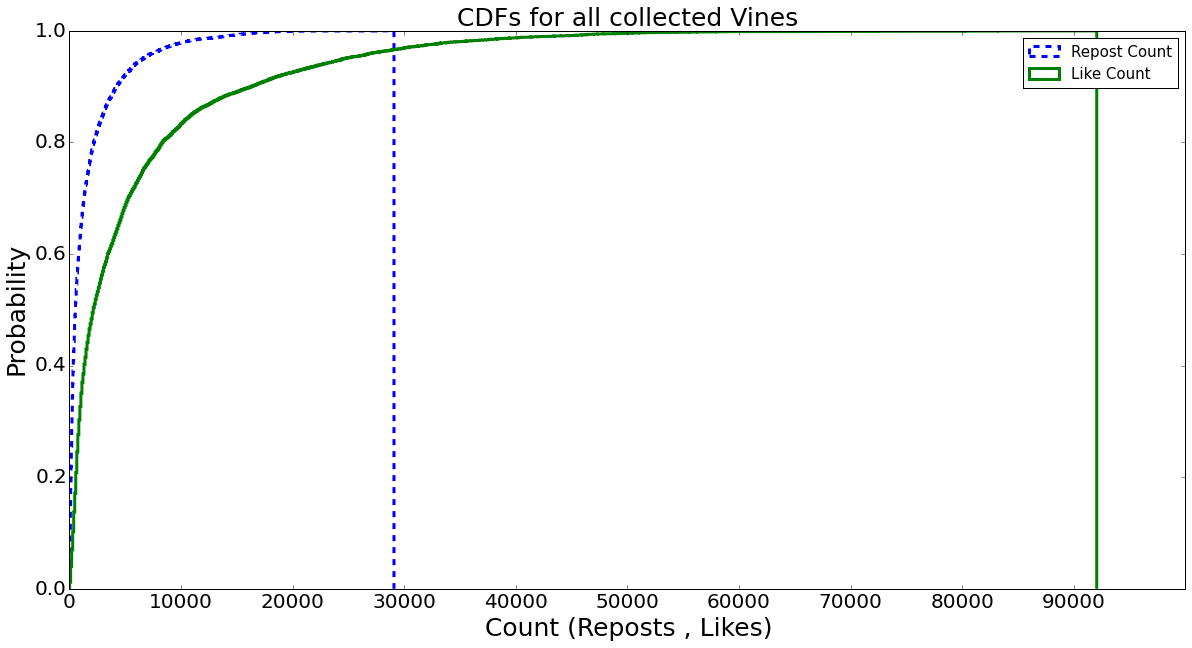
\includegraphics[width=\columnwidth]{plots/Like_repost_CDF}
\caption{\textbf{CDF of likes and repost count across collected Vines.}}
\label{fig:Like_Repost_CDF}
\end{figure}